%%This is a very basic article template.
%%There is just one section and two subsections.
\documentclass{article}
\usepackage[MeX]{polski} 		%linkuje pakiet polski
\usepackage[utf8]{inputenc}	%ustawia kodowanie
\usepackage{latexsym}			%znaczki matematyczne
\usepackage{indentfirst}		%akapity zaczynaja sie od wciecia
\usepackage{wasysym}
\usepackage{graphicx}
\usepackage{fancyhdr}
%%\usepackage{pxfonts}
\usepackage{url}
\usepackage{clrscode}			%pseudokod
\usepackage{array}
\usepackage{amssymb}				%symbole
\author{Łukasz Wojnarowski (80164)\\ Tomasz Kujawa (75909)}
\title{Techniki optymalizacji}

\setlength{\textheight}{22cm}
\setlength{\textwidth}{15.72cm}
\setlength{\footskip}{10mm}
\setlength{\oddsidemargin}{0mm}
\setlength{\evensidemargin}{0mm}
\setlength{\topmargin}{0mm}

%%\let\stdsection\section
%%\renewcommand\section{\newpage\stdsection}

\begin{document}

\pagestyle{empty}
\pagestyle{fancy}
\renewcommand{\sectionmark}[1]{\markright{\thesection \quad #1}}
\fancyhf{}
\fancyhead[LE,RO]{\small\bfseries\thepage}
\fancyhead[LO]{\small\bfseries\rightmark}
\renewcommand{\headrulewidth}{0.5pt}
\renewcommand{\footrulewidth}{0pt}
\addtolength{\headheight}{0.5pt}
\fancypagestyle{plain}{
\fancyhead{}
\renewcommand{\headrulewidth}{0pt}
}

\maketitle
\newpage
\tableofcontents %spis treœci
\newpage

\section{Opis problemu}
Rozwiązywany problem jest rozwinięciem \emph{problemu komiwojażera} (TSP - ang. traveling salesman problem), który polega na znalezieniu 4 cykli hamiltona w pełnym grafie ważonym o minimalnej sumie wag.

Dane wejściowe składają się z grafu pełnego $\mathcal{G}=(\mathcal{V},\mathcal{E})$, gdzie $\mathcal{V}$ to zbiór wierzchołków (można go interpretować jako zbiór punktów na płaszczyźnie), a $\mathcal{E}$ to zbiór krawędzi.
Dla każdej z krawędzi $\{v_i,v_j\} \colon v_i,v_j \in \mathcal{V}$ znana jest waga, będąca odległością pomiędzy wierzchołkami $v_i,v_j$. Rozwiązaniem problemu są cztery cykle proste
\begin{equation}
w_1,w_2,w_3,\ldots,w_{n-1},w_n \mbox{ ; }x_1,x_2,x_3,\ldots,x_{n-1},x_n \mbox{ ; } y_1,y_2,y_3,\ldots,y_{n-1},y_n \mbox{ oraz } z_1,z_2,z_3,\ldots,z_{n-1},z_n,
\end{equation} które spełniają następujące ograniczenia:
\begin{itemize}
	\item $w_i \in \mathcal{V'}$,
	\item $x_j \in \mathcal{V''}$,
	\item $y_k \in \mathcal{V'''}$,
	\item $z_l \in \mathcal{V''''}$,
	\item $\mathcal{V'} \cup \mathcal{V''} \cup \mathcal{V'''} \cup \mathcal{V''''} = \mathcal{V}$,
	\item $\mathcal{V'} \cap \mathcal{V''} \cap \mathcal{V'''} \cap \mathcal{V''''} = \varnothing$,
	\item $|\mathcal{V'}| = |\mathcal{V''}| = |\mathcal{V'''}| = |\mathcal{V''''}| = n$, przy założeniu, że $\mathcal{V} = 4n$.
\end{itemize}

Niech $|{v_i, v_j}|$ oznacza wagę (koszt przebycia drogi) krawędzi pomiędzy wierzchołkami $v_i, v_j$. Dla tak zdefiniowanego modelu funkcja celu została określona w następujący sposób:
\begin{equation}
min C = \sum \limits_{i<n}^{i=1} |w_i,w_{i+1}| + |w_n,w_1| + \sum \limits_{i<n}^{i=1} |x_i,x_{i+1}| + |x_m,x_1| + \sum \limits_{i<n}^{i=1} |y_i,y_{i+1}| + |y_m,y_1| + \sum \limits_{i<n}^{i=1} |z_i,z_{i+1}| + |z_m,z_1|
\end{equation}

gdzie $|\mathcal{V}| = 4n$.

\section{Generowanie rozwiązania początkowego (\emph{RP})}
\subsection{Opis metody} \label{sec:rp_section}
Analizowana metoda generowania rozwiązania początkowego to \emph{grupowanie} i następnie \emph{poszukiwanie najbliższego sąsiada}.

\subsubsection{Słowny} \label{sec:slownyrp}
Metoda rozpoczyna się od losowego wybrania wierzchołka początkowego, na którego podstawie stworzone zostaną grupy. Grupy mają najpierw przydzielane z puli dostępnych wierzchołków elementy początkowe - takie, że środek ciężkości od punktów już wcześniej przydzielonych jest największy. Następnie na podstawie wybranych "liderów" budowane są grupy - tak, że każdy kolejny element dodawany do grupy będzie miał najmniejszą odległość od środka ciężkości grupy. Należy zaznaczyć, że przydział po grupach odbywa się iteracyjnie - tzn. najpierw przydzielamy jeden element do grupy pierwszej, potem jeden element do grupy drugiej i iteracyjnie aż do wyczerpania się elementów nieprzydzielonych do żadnej grupy. Przydział ten jest powtarzany, aż stworzone zostaną 4 grupy o równych licznościach.

Następnie w każdej grupie następuje budowanie ścieżki (cyklu) tak, że przy każdym kroku wybierany jest taki wierzchołek, że jego odległość od środka ciężkości dotychczas wybranych wierzchołków jest najmniejsza. Algorytm zatrzymuje się, jeśli w grupie nie będzie już nieodwiedzonych wierzchołków. Należy pamiętać, by rozwiązanie uzupełnić o krawędź pomiędzy ostatnim a pierwszym wierzchołkiem - tzn. by waga zwracana uwzględniała połączenie pomiędzy ostatnim, a pierwszym elementem cyklu.

\newpage
\subsubsection{Pseudokod}

Poniżej zaprezentowano pseudokod algorytmu opisanego w części \ref{sec:slownyrp}.

\begin{codebox}
	\Procname{$\proc{Generuj rozwiązanie początkowe}(\mathcal{V})$}
	\li $\proc{Generuj podział na grupy}()$
	\li
	\li $\id{i} \gets 1$
	\li \For  \emph{$\forall$ $\id{i}$ in $\{1, 2, 3, 4\}$}
		\li \Do
			\li $\id{v} \gets \proc{Pobierz losowy z grupy}(\id{i})$
			\li $\proc{Przydziel wierzchołek do ścieżki w grupie}(\id{v})$
		\li \End
	\li \While \emph{$\exists$ grupa z nieprzydzielonymi wierzchołkami}
	\li \Do
		\li $\id{next} \gets \proc{Najbliższy nieprzydzielony wierzchołek dla grupy}(\id{i})$
		\li $\proc{Przydziel wierzchołek do ściezki w grupie}(next)$
		\li $i=(i+1) \% 5$
		\li \End
	\End
\end{codebox}

W kodzie wykorzystano metode przygotowania grup, która została zaprezentowana poniżej:


\begin{codebox}
	\Procname{$\proc{Generuj podział na grupy}(\mathcal{V})$}
	\li $\id{v1} \gets  \proc{Pobierz losowo}(\mathcal{V})$
	\li $\id{v2} \gets  \proc{Pobierz najdalszy}(\mathcal{V} \setminus\{\id{v1}\} )$
	\li $\id{v3} \gets  \proc{Pobierz najdalszy}(\mathcal{V} \setminus\{\id{v1, v2}\} )$
	\li $\id{v4} \gets  \proc{Pobierz najdalszy}(\mathcal{V} \setminus\{\id{v1, v2, v3}\} )$
	\li $\proc{Umieść wierzchołek w grupie}(\id{v1}, $1$)$
	\li $\proc{Umieść wierzchołek w grupie}(\id{v2}, $2$)$
	\li $\proc{Umieść wierzchołek w grupie}(\id{v3}, $3$)$
	\li $\proc{Umieść wierzchołek w grupie}(\id{v4}, $4$)$
	
	\li $\id{i} \gets 1$
	\li \While \emph{$\exists$ $\mathcal{U} \gets $ wierzchołki nieumieszczone w żadnej grupie}
	\li \Do
		\li $\id{closest\_v} \gets \proc{Pobierz najbliższy do \id{i}-tej grupy }(\mathcal{U})$
		\li $\proc{Umieść w grupie}(\id{closest\_v}, $i$)$
		\li $i=(i+1) \% 5$
		\li \End
\end{codebox}

\section{Losowe rozwiązanie początkowe - LRP}
Opisane w poprzednim rozdziale RP porównywane było z generowanym losowo podziałem na grupy. Pozwoliło to już na etapie kreacji grup zauważyć, jak ważne jest poszukanie odpowiedniej metody przygotowania rozwiązania początkowego. 

Ponieważ rozwiązanie to jest proste i intuicyjne pominięto opis - zarówno w pseudokodzie, jak i słowny. Należy tylko odnotować, że w programie jest porównywanie rozwiązania \emph{RP} z losowym rozwiązaniem początkowym.

\subsection{Wyniki}

W tabeli \ref{tab:wynikirp} zostały przedstawione uśrednione wyniki dla opracowywanej metody.

\begin{table}[h!]
\begin{center}
  
  \begin{tabular}{| c | c | m{3cm} | c | c | c | }
    \hline
	instancja & \centering metoda & śr. wart. roz. z 10 pomiarów & mediana & odch. std. & najlepsza wartość \\ \hline
    kroA100.txt & NS G & \centering 33 721 & 33 174 & 3 551 & 26 742\\
      & LRP & \centering 171 479 & 170 055 & 9 635 & 153 474\\
    \hline
    kroB100.txt & NS G & \centering 35 210 & 25 979 & 3 393 & 30 173\\
      & LRP & \centering 166 257 & 166 053 & 6 220 & 153 757\\
    \hline
  \end{tabular}
\end{center}
\caption{Uśrednione wyniki pomiarów.} \label{tab:wynikirp}
\end{table}

\begin{figure}[h!]
\centering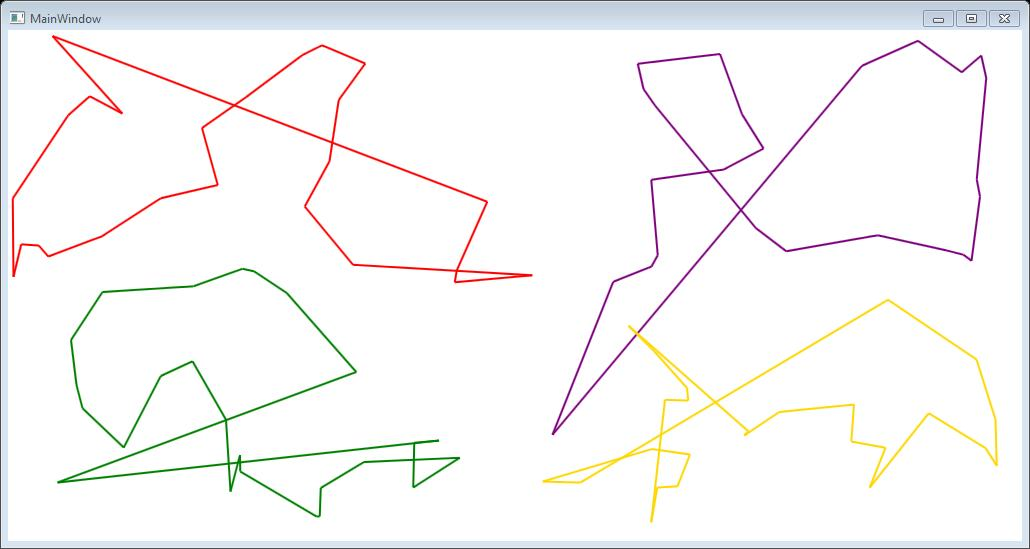
\includegraphics[width=17cm]{img/rys1.png}
\caption{Rozwiązanie początkowe dla \emph{kroA100.txt}}
\end{figure}

\section{Local search (LS)}
\subsection{Opis metody}
Analizowana metoda generowania rozwiązania to \emph{rozrywanie (1 ruch) w wersji stromej}.

\subsection{Opis słowny metody}
Proces poszukiwania lokalnego optimum rozpoczyna się od wykonania kroków z opisanego w rozdziale \emph{Generowanie rozwiązania początkowego}. Następnie na takim rozwiązaniu dokonywane jest lokalne przeszukiwanie.

Kroki metody:
	\begin{enumerate}
		\item Wybierz wierzchołek i $k-1$ mu najbliższych wierzchołków. 
		\item Rozerwij łuki wokół tych wierzchołków.
		\item Rozważ wszystkie możliwe sposoby naprawy do rozwiazania tego problemu.
		\item Wykonaj ruch, który przynosi najwięcej zysku.
	\end{enumerate}

Parametr $k \in {2,3,4}$ jest definiowany na wejściu programu.

\subsection{Pseudokod}
Algorytm generowania rozwiązania można zapisać przy pomocy poniższego pseudokodu.
\begin{codebox}
	\Procname{$\proc{Lokalne przeszukiwanie}(\mathcal{V}, \id{k})$}
	\li $\id{rozwiązanie} \gets  \proc{Generuj rozwiązanie początkowe}(\mathcal{V})$
	\li \While (\const{true})
	\li \Do 
	\li $\id{zysk} \gets 0 $
	\li $\id{wybrani} \gets \proc{Wybierz łuki} (\id{k}, \mathcal{V}) $
	\li $\id{możliwe\_przydziały} \gets \proc{Generuj możliwe przydziały} (\id{wybrani}) $
	\li $\id{wartość} \gets \proc{Oblicz wartość rozwiązania} (\id{rozwiązanie}) $
	\li \For  \emph{$\forall$ $\id{ruch}$ in $\id{możliwe\_przydziały}$}
		\li \Do
				\li $\id{aktualne\_rozwiązanie} \gets \proc{Wykonaj ruch} (\id{rozwiązanie}, \id{ruch}) $
				\li $\id{aktualna\_wartość} \gets \proc{Oblicz wartość rozwiązania} (\id{aktualne\_rozwiązanie}) $
				\li $\id{aktualny\_zysk} \gets \id{wartość} - \id{aktualna\_wartość}) $
				\li \If $\id{aktualny\_zysk} \geq \id{zysk}$
					\li \Then
						\li $\id{zysk} \gets  \id{aktualny\_zysk}$
						\li $\proc{Zapamiętaj ruch}(\id{ruch})$
					\li \Else
						\li \Return
					 \End
			\End
	\li
	\li \If $\id{zysk} > 0$
		\li \Then
			\li $\proc{Wykonaj zapamiętany ruch}(\id{rozwiązanie})$
		\li \Else
			\li \Return
		 \End
	\li \End
	
\end{codebox}

\subsection{Wyniki}
W tabeli przedstawione zostały zbiorcze wyniki pomiarów:
\begin{itemize}
	\item \emph{RP} - metoda z pierwszego ćwiczenia - generowanie rozwiązania początkowego,
	\item \emph{RP + LS} - metoda lokalnego przeszukiwania rozpoczynająca się od wygenerowania rozwiązania początkowego zgodnie z zasadami z ćwiczenia numer 1,
	\item \emph{LRP + LS} - metoda lokalnego przeszukiwania rozpoczynająca się od wygenerowania losowego rozwiązania początkowego zgodnie z zasadami z ćwiczenia numer 2.
\end{itemize}
	
\newcolumntype{S}{>{\centering\arraybackslash} m{3cm} }
\newcolumntype{D}{>{\centering\arraybackslash} m{5cm} }

\begin{table}[h!]
\begin{center}
\centering
  \begin{tabular}{| c | D | S | c | S | }
\hline
	instancja & metoda & śr. jakość (odch. standardowe) & śr. czas [ms] & jakość najlepszego przeszukiwania \\ \hline
    kroA100.txt & \emph{RP} & 33 721 (3 551) & 0 & 26 742 \\
     & \emph{RP + LS} & 32 417 (3 508) & 423 & 25 604 \\
     & \emph{LRP} & 171 479 (9 635) & 0 & 153 474 \\
     & \emph{LRP + LS} & 152 039 (9 376) & 620 & 127 767 \\
\hline
    kroB100.txt & \emph{RP} & 35 210 (3 393) & 0 & 35 979 \\
     & \emph{RP + LS} & 34 305 (3180) & 363 & 29 428 \\
     & \emph{LRP} & 166 257 (6 220) & 0 & 153 757 \\
     & \emph{LRP + LS} & 145 413 (8 695) & 733 & 148 168 \\
\hline
  \end{tabular}
\end{center}
\caption{Uśrednione wyniki pomiarów.} \label{tab:wynikils}
\end{table}

\begin{figure}[h!]
\centering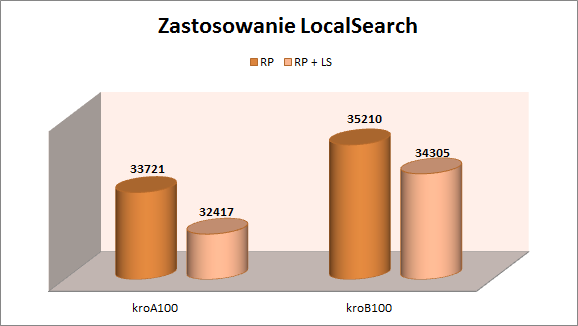
\includegraphics[width=13cm]{img/wyk2.png}
\caption{Wyniki eksperymentów - zastosowanie LocalSearch do poprawy jakości rozwiązania generowanego przez RP}
\label{wyk:wyniki_ls_rp}
\end{figure}

\begin{figure}[h!]
\centering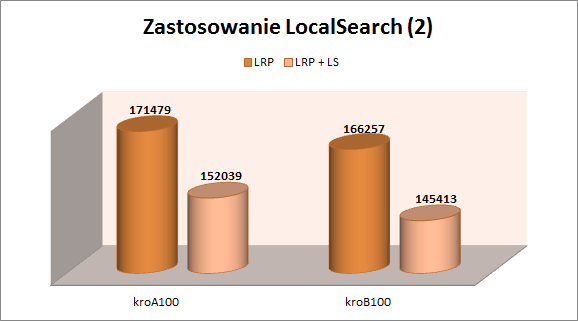
\includegraphics[width=13cm]{img/wyk3.png}
\caption{Wyniki eksperymentów - zastosowanie LocalSearch do poprawy jakości rozwiązania generowanego przez LRP}
\label{wyk:wyniki_ls_lrp}
\end{figure}

Rysunki \ref{wyk:wyniki_ls_rp} oraz \ref{wyk:wyniki_ls_lrp} prezentują kolejno wyniki zastosowania LocalSearch do optymalizacji rozwiązania generowanego przez RP (rys.\ref{wyk:wyniki_ls_rp}, a także LRP (rys.\ref{wyk:wyniki_ls_lrp}). Analizując dane łatwo zauważyć, że przy generowaniu rozwiązania metodą RP zastosowanie LS przynosi jedynie niewielką poprawę rozwiązania - na poziomie $4-5\%$. Wynika z tego, że przyjęty sposób generowania rozwiązania początkowego (zobacz rozdział \ref{sec:rp_section}) generuje bardzo dobre rozwiązanie początkowe - w sensie lokalnej jego optymalizacji.

Lepszą poprawe zaobserwować można na wykresie \ref{wyk:wyniki_ls_lrp}, gdzie zastosowanie LS poprawiało wynik generowany przy pomocy LRP o około $13\%$.

\subsection{Rysunki najlepszych rozwiązań}
Na poniższych rysunkach przedstawione zostały rozwiązania wygenerowane przy pomocy metody \emph{RP + LS}.
\begin{figure}[h!]
\centering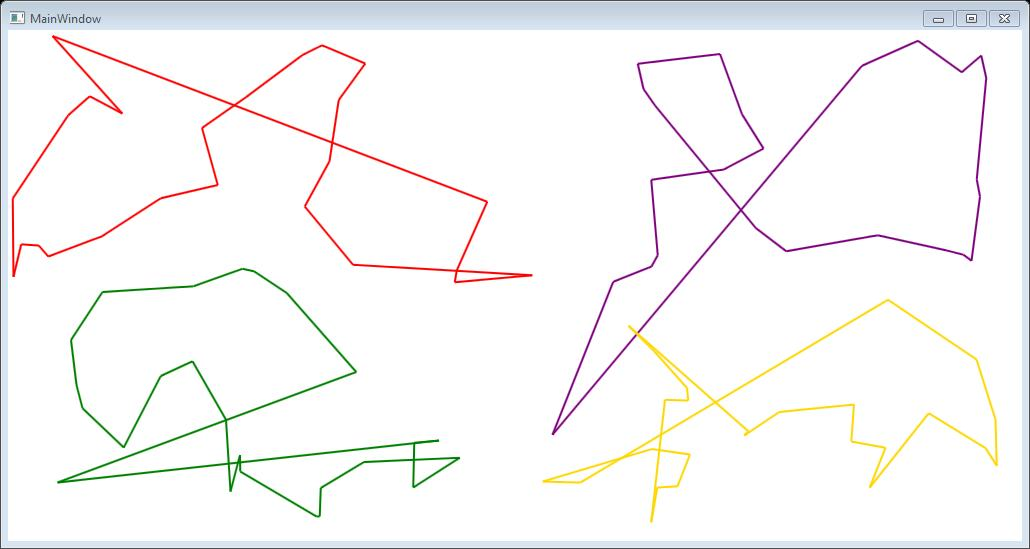
\includegraphics[width=17cm]{img/rys2.png}
\caption{Rozwiązanie RP+LS dla \emph{kroA100.txt}}
\end{figure}
\begin{figure}[h!]
\centering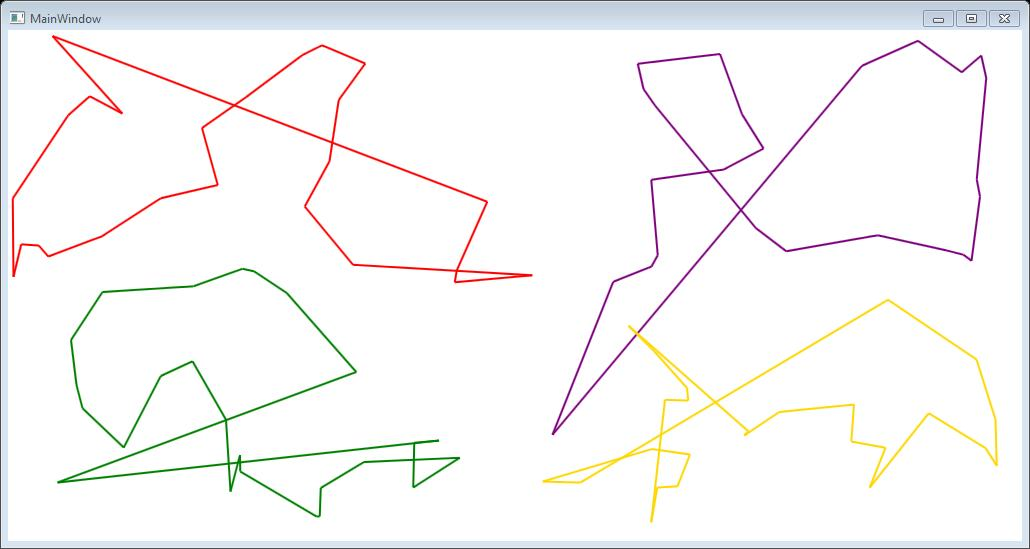
\includegraphics[width=17cm]{img/rys3.png}
\caption{Rozwiązanie RP+LS dla \emph{kroB100.txt}}
\end{figure}


\section{Heurystyczny Algorytm Ewolucyjny (HEA)}
\subsection{Wstęp}
W ramach wykonania zadania przygotowano implementację Heurystycznego Algorytmu Ewolucyjnego dla problemu komiwojażera.

W kolejnych podrozdziałach przygotowano opis słowny, a także pseudokod rozwiązania w ramach opracowywanego zadania. 

\subsection{Opis słowny metody}
Algorytm rozpoczyna się od wygenerowania pewnej populacji początkowej - przeprowadzane są kroki opisane we wcześniejszych roździałach. Oprócz wykorzystania LS przy budowie wstępnej populacji, wykorzystuje się go również do optymalizacji rozwiązań otrzymywanych w populacji rozwiązań po przeprowadzaniu mutacji.

Kroki algorytmu powtarzane są do momentu, w którym przekroczony zostanie dostępny na obliczenia czas - który to jest parametrem wejściowym do algorytmu. W testach (zgodnie z poleceniem prowadzącego) przyjęto wartość 30 sekund (bądź 60, dla bardziej rozbudowanego zestawu danych testowych). 

Pierwszy krok, to wybór rozwiązań z populacji rozwiązań, które poddawane będą ewolucji. Dokonuje się to przy pomocy losowego wyborów elementów dostępnych w populacji. Należy podkreślić, że liczba wybranych rozwiązań jest parametrem definiowalnym dla algorytmu.

Drugi krok to dokonanie rekombinacji na parach (losowo dobieranych) z rozwiązań wybranych w kroku poprzednim.

Następny krok to mutacja, którą logicznie można podzielić na dwa etapy:
	\begin{itemize}
		\item \emph{premutacja} - czyli opracowanie wstępnych rozwiązań na podstawie dostarczonych list wspólnych ścieżek dla par rozwiązań,
		\item \emph{właściwa mutacja} - czyli losowe wypełnienie brakujących połączeń punktami, które nie znajdują się na żadnej ze wspólnych scieżek.
	\end{itemize}
	
Każdy z tych etapów może być konfigurowalny parametrami, które definiują liczbę generowanych rozwiązań na poszczególnych etapach. Pozwala to w elastyczny sposób zarządzać przestrzenią rozwiązań, tak by nie rozrastała się ona w zbyt szybkim tempie.

Ostatni etap, to ograniczenie przestrzeni rozwiązań, tak by nie rozrastała się ona w zbyt intensywnym tempie - chodzi o ograniczenia pamięciowe poszczególnych maszyn testowych. Także i w tym wypadku definiuje się parametr wejściowy, który określa maksymalny rozmiar populacji rozwiązań algorytmu ewolucyjnego.

\subsection{Pseudokod}
Wcześniej zdefiniowane wartości:
	
\begin{codebox}
	\li $\id{max\_rozmiar\_populacji}$
	\li $\id{liczba\_rozwiązań\_do\_ewolucji}$
	\li $\id{liczba\_premutacji}$
	\li $\id{liczba\_mutacji}$
\end{codebox}

Ogólna idea heurystycznego algorytmu ewolucyjnego zaimplementowanego w ramach wykonywania zadania:

\begin{codebox}
	\Procname{$\proc{Heurystyczny Algorytm Ewolucyjny}(\mathcal{V}, \id{max\_czas})$}
	\li $\id{populacja\_rozwiązań} \gets  \proc{Generuj populację początkową}(\mathcal{V})$
	\li \While (\const{true})
	\li \Do 
	\li $\id{do\_ewolucji} \gets \proc{Wybór rozwiązań do ewolucji} (\id{populacja\_rozwiązań})  $
	\li $\id{wspólne\_ściezki} \gets \proc{Rekombinacja losowych par} (\id{do\_ewolucji}) $
	\li $\id{dodatkowa\_populacja} \gets \proc{Mutacja} (\id{wspólne\_ścieżki}, \id{pozostałe\_punkty}) $
	\li $\id{dodatkowa\_populacja} \gets \proc{Lokalne przeszukiwanie na populacji}(\id{dodatkowa\_populacja})$
	\li $\id{populacja\_rozwiązań} \gets \id{populacja\_rozwiązań} \cup \id{dodatkowa\_populacja} $
	\li $\proc{Ograniczenie przestrzeni rozwiązań} (\id{populacja\_rozwiązań}) $
	\li \If $\id{czas\_trwania\_algorytmu} > \id{czas}$
		\li \Then
			\li $\proc{Przerwij algorytm}()$
		\End
	\li \End
	\li $\id{rezultat} \gets \proc{Wybór najlepszego rozwiązania} (\id{populacja\_rozwiązań})$	
	
\end{codebox}

\subsection{Eksperymenty i wyniki}
W tabeli przedstawione zostały zbiorcze wyniki pomiarów:
\begin{itemize}
	\item \emph{RP + LS} - metoda lokalnego przeszukiwania rozpoczynająca się od wygenerowania rozwiązania początkowego zgodnie z zasadami z ćwiczenia numer 1,
	\item \emph{RP + HEA} - metoda heurystycznego algorytmu ewolucyjnego z wykorzystaniem algorytmu lokalnego przeszukiwania. 
\end{itemize}
	
\newcolumntype{S}{>{\centering\arraybackslash} m{3cm} }
\newcolumntype{D}{>{\centering\arraybackslash} m{5cm} }

\begin{table}[h!]
\begin{center}
\centering
  \begin{tabular}{| c | D | S | c | S | }
\hline
	instancja & metoda & śr. jakość (odch. standardowe) & śr. czas [ms] & jakość najlepszego przeszukiwania \\ \hline
    kroA100.txt & \emph{RP + LS} & 32 417 (3 508) & 423 & 25 604 \\
     & \emph{RP + HEA} & 25 181 (95) & 30 000 & 25 061 \\
\hline
    kroB100.txt & \emph{RP + LS} & 34 305 (3180) & 363 & 29 428 \\
     & \emph{RP + HEA} & 27 649 (530) & 30 000 & 26 446 \\
\hline
    kroA150.txt & \emph{RP + LS} & 44 193 (3 765) & 503 & 36 629 \\
     & \emph{RP + HEA} & 34 898 (266) & 60 000 & 34 420 \\
\hline
  \end{tabular}
\end{center}
\caption{Uśrednione wyniki pomiarów - porównanie efektywności algorytmu heurystycznego w stosunku do zastosowania lokalnego przeszukiwania.} \label{tab:wynikils}
\end{table}

\begin{figure}[h!]
\centering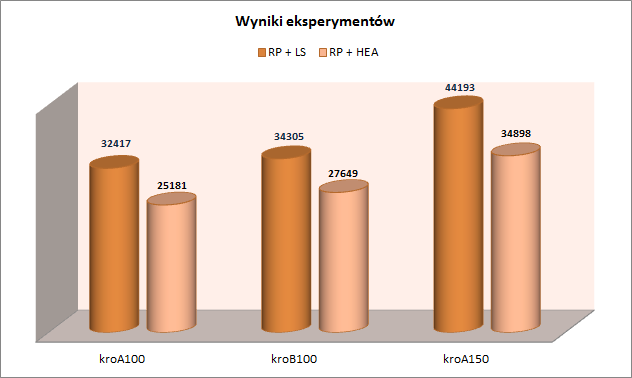
\includegraphics[width=17cm]{img/wyk1.png}
\caption{Wyniki eksperymentów}
\label{wyk:wyniki}
\end{figure}

Należy zauważyć, że zbiór \emph{kroA150.txt} zawierał 150 punktów - ponieważ w założeniach do zadania przyjęto, że zbiór powinien móc podzielić się na 4 równe podzbiory (podgrupy) - przyjęto, że do zadania skierowane zostanie pierwsze 148 punktów ze zbioru.

Na rysunku \ref{wyk:wyniki} przedstawiony został wykres z pomiarów. Łatwo zauważyć, że algorytm HEA wykazuje około $20\%$ "zysk" w stosunku do zastosowania jedynie algorytmu lokalnego przeszukiwania - dla każdego z zestawów są to wartości bliskie takiemu współczynnikowi.

\end{document}
